\documentclass{article}
\usepackage[utf8]{inputenc}
\usepackage[T1]{fontenc}
\usepackage{graphicx}
\usepackage{hyperref}
\usepackage{geometry}
\geometry{margin=1in}

\title{ERFURT}
\date{Encyclopaedia Britannica (1771)}

\begin{document}
\maketitle

\section*{Historical source}
\textbf{Entry ID:} \texttt{entry-erfurt-2473} \\
\textbf{Volume ID:} 144133902 \\
\textbf{Character Count:} 147

\subsection*{Extracted Text}
ERFURT, a large and beautiful city of Upper Saxony in Germany, capital of Thailand, and subject to the elckor of Menus; E. long.117 é', N.lax. 910.



\section*{Source record}
\begin{itemize}
\item \textbf{Dataset:} \texttt{NationalLibraryOfScotland/encyclopaedia\_britannica\_illustrated}
\item \textbf{Dataset Revision:} \texttt{309f765b1ecc83e0a7f7762e44b4a927a7555443}
\item \textbf{Page ID:} \texttt{britannica:309f765b1ecc83e0a7f7762e44b4a927a7555443:train:2473} \\
  \textbf{Filename:} \texttt{page-2473-b849fb7f25f2.jpg} \\
  \textbf{Row Index:} 2473 \\
  \textbf{SHA256:} \texttt{b849fb7f25f25b39...}
\end{itemize}

\begin{figure}[h]
\centering
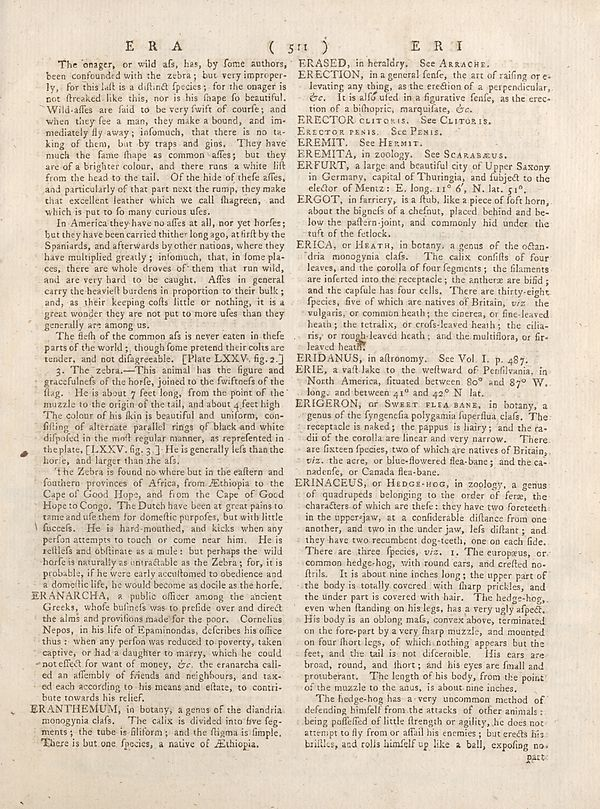
\includegraphics[width=0.85\textwidth]{../scans/page-2473-b849fb7f25f2.jpg}
\caption*{Source scan: \texttt{page-2473-b849fb7f25f2.jpg}}
\end{figure}

\end{document}
